%TCIDATA{LaTeXparent=0,0,relatorio.tex}



\chapter{Desenvolvimento\label{chap:Desenvolvimento}}

% Resumo opcional. Comentar se não usar.
\resumodocapitulo{``Só sei que nada sei'' -- Plato}

\section{Introdução}

Este capítulo irá apresentar as soluções adotadas para os problemas de planejamento de tarefas e de tomada de decisões, junto com sua modelagem matemática. Aqui também serão descritos os ambientes de teste em simulação e a modelagem utilizada para descrever o agente móvel.

\section{Modelagem Matemática}

Nessa seção iremos descrever as mudanças que foram feitas nos modelos matemáticos utilizados nesse projeto. Faremos também uma explicação de como ficou o modelo final do projeto e de como as várias teorias se encaixam.

\subsection{Aprendizagem por Reforço para Seleção de Comportamentos} \label{subsection:QLearningSelecaoDeComportamento}

Nesse trabalho, queremos utilizar a aprendizagem por reforço para aprender uma política de seleção de comportamento e não de ações. Para isso nós devemos alterar as equações do algoritmo Q Learning para, ao invés de escolher uma ação $ u \in U $, escolher um comportamento $ b \in B $. Reescrevendo as principais equações desse algoritmo elas são:

\begin{equation} \label{equation:QValueFunctionBehavior}
    Q^t \left( s, b \right) = \int \! \left( r \left( s, b, s' \right) + \gamma \cdot V^{t-1} \left( s' \right) \right) \cdot P \left( s' \mid b, s \right) \, \mathrm{d}s'
\end{equation}


\begin{equation} \label{equation:PolicySelectionBehavior}
    \pi^t \left( s \right) = \underset{b}{argmax} \left( Q^t \left( s, b \right) \right)
\end{equation}

\begin{equation}
    V^t \left( s \right) = \underset{b}{max} \left( Q^t \left( s, b \right) \right)
\end{equation}

Além disso, nossas características $ f_j $ agora devem ser baseadas em pares estado-comportamento $ \left( S, B \right) $ e não em pares estado-ação.

\begin{equation}
	Q \left( S, B \right) = \omega_1 \cdot f_1 \left( S, B \right) + \omega_2 \cdot f_2 \left( S, B \right) + \cdots + \omega_n \cdot f_n \left( S, B \right)
\end{equation}

\begin{equation} \label{equation:QErrorBehavior}
	erro = r \left( s, b, s' \right) + \gamma \cdot \underset{b}{max} \left( Q^{t-1} \left( s', b' \right) \right) - Q^{t-1} \left( s, b \right)
\end{equation}

\begin{equation} \label{equation:OmegaUpdateBehavior}
	\omega_i^t = \omega_i^{t-1} + \alpha \cdot erro \cdot f_i \left( s, b \right)
\end{equation}


\subsection{Seleção de Comportamentos em um Sistema Parcialmente Observável} \label{subsection:QLearningParcialmenteObservavel}

O algoritmo Q Learning foi criado baseado num MDP, que, como citado na seção \ref{section:MDP}, é ultilizado para sistemas completamente observáveis%
\footnote{Sistemas em que existe uma função $ f \left( Z \right) $ que, dado uma medida dos sensores, retorna o estado atual do sistema. Em outras palavras, é um sistema em que, dado uma medida $ z \in Z $ dos sensores se sabe, sem dúvidas, qual o estado presente do sistema $ s \in S $%
}. Temos, então, de expandir sua definição para aplicá-lo em um sistema parcialmente observável%
\footnote{Sistema que não é completamente observável, ou seja, que para uma medida $ z \in Z $ dos sensores só se pode estimar qual a probabilidade desse sistema se encontrar num estado $ s \in S $%
}.

Para isso precisamos primeiramente introduzir uma nova variável $ a \in A $ que representa a distribuição de probabilidades nos possíveis estados $ S $. Considere, por exemplo, um caso em que o estado seja dado por duas variáveis $ S = \binom{S_1}{S_2} $ que podem ter valores $ S_1 \in \left\{1,2,3\right\} $ e $ S_2 \in \left\{verdadeiro, falso\right\} $. Uma variável $ a \in A $, nesse caso, seria dada por cinco variáveis, representando as probabilidades de S ter cada um dos possíveis valores.

$$
	A = \left(
	\begin{matrix}
		P \left( S_1 = 1 \right) & P \left( S_2 = verdadeiro \right) \\
		P \left( S_1 = 2 \right) & P \left( S_2 = falso \right) \\
		P \left( S_1 = 3 \right) &  
	\end{matrix} \right)
$$

Tendo posse dessa definição, utilizando como inspiração o algoritmo POMDP [refs POMDP], podemos substituir na equação \ref{equation:QValueFunctionQLearning} o estado $ s \in S $ por uma variável $ a \in A $ que represente essa distribuição de probabilidades nos possíveis estados $ S $.

\begin{equation} \label{equation:QValueFunctionPartiallyObservable}
    Q^t \left( a, b \right) = \int \! \left( r \left( a, b, a' \right) + \gamma \cdot V^{t-1} \left( a' \right) \right) \cdot P \left( a' \mid b, a \right) \, \mathrm{d}a'
\end{equation}

E agora temos uma seleção de política baseada na distribuição de probabilidades nos estados $ s \in S $:

\begin{equation} \label{equation:PolicySelectionPartiallyObservable}
    \pi^t \left( a \right) = \underset{b}{argmax} \left( Q^t \left( a, b \right) \right)
\end{equation}

\begin{equation}
    V^t \left( a \right) = \underset{b}{max} \left( Q^t \left( a, b \right) \right)
\end{equation}


Analogamente às equações \ref{equation:AmostraQLearning} e \ref{equation:QUpdateQLearning} no Q Learning normal, aprende-se através de amostras obtidas a partir de experiências $ \left( a, b, a', r \right) $.


\begin{equation}
	amostra = r \left( a, b, a' \right) + \gamma \cdot \underset{b}{max} \left( Q^{t-1} \left( a', b' \right) \right)
\end{equation}

\begin{equation}
	Q^t \left( a, b \right) = \left( 1 - \alpha \right) \cdot Q^{t-1} \left( a, b \right) + \alpha \cdot amostra
\end{equation}

O problema com essa equação é que, ao utilizar um espectro $ a \in A $ de probabilidades de todos os estados $ s \in S $, no lugar do próprio estado, não podemos simplesmente aprender os valores para cada item. Isso acontece pois, mesmo para espaços de estados discretos, teremos infinitos valores de $ a \in A $ possíveis.

Vamos, então, utilizar a teoria vista no tópico \ref{subsection:GeneralizaçãoParesEstadoAção} para criar uma generalização desses estados através de características deles. Essas características, ao contrário das vistas anteriormente, devem ser baseadas nas probabilidades de se estar/alcançar um estado. Alguns exemplos seriam:

\begin{itemize}
	\item Distância da posição mais provável do robô, para uma posição que ofereça um produto ( probabilidade de receber uma recompensa * recompensa ) alta;
	\item Distância da posição mais provável do robô, para uma posição que ofereça um produto ( probabilidade de receber uma recompensa * recompensa ) negativa;
	\item Probabilidade de existir algum perigo (recompensa negativa) a menos que uma certa distância;
	\item Probabilidade de capturar um alvo;
	\item Porcentagem de chance do robô ter um erro.
\end{itemize}

Essas características podem, como no caso anterior, descrever também o comportamento a ser executado, como:

\begin{itemize}
	\item Tenta capturar um alvo;
	\item Tenta fugir de um perigo;
	\item Economiza energia.
\end{itemize}

Com isso obtemos um valor $ Q \left( A, B \right) $ tal que:

\begin{equation}
	Q \left( A, B \right) = \omega_1 \cdot f_1 \left( A, B \right) + \omega_2 \cdot f_2 \left( A, B \right) + \cdots + \omega_n \cdot f_n \left( A, B \right)
\end{equation}


Com esse novo modelo, podemos aprender valores, a partir de cada experiência, utilizando o erro atual do modelo:

\begin{equation} \label{equation:ErroQPartiallyObservable}
	erro = r \left( a, b, a' \right) + \gamma \cdot \underset{b}{max} \left( Q^{t-1} \left( a', b' \right) \right) - Q^{t-1} \left( a, b \right)
\end{equation}

E o utilizando para atualizar cada um dos pesos usados para obter $ Q^t \left( A, B \right) $:

\begin{equation} \label{equation:UpdateOmegaQPartiallyObservable}
	\omega_i^t = \omega_i^{t-1} + \alpha \cdot erro \cdot f_i \left( a, b \right)
\end{equation}

Assim, caso tenhamos um erro grande para um dado espectro de probabilidades, iremos atualizar os valores de todos os casos que possuam espectros de probabilidades dos estados com características similares àquele. E caso esse estado tenha um valor maior para uma das características, o peso dela será mais modificado que as outras.

O que isso significa é que, por exemplo, se estiver utilizando como característica $ f_i = $ ``probabilidade de existir algum perigo (recompensa negativa) a menos que uma certa distância''. Caso se receba uma recompensa negativa num estado em que o valor de $ f_i $ é alto, estados com essa característica serão considerados piores. No caso de se receber uma recompensa positiva, pode-se considerar estados com essa característica como bons.


\subsection{Abordagem Bayesiana com a Seleção de Comportamentos} \label{subsection:BayesComSelecaoDeComportamento}

Partindo dos modelos obtidos na seção \ref{section:FiltroBayesiano}, podemos agora utilizar a seleção de comportamento, vista no tópico \ref{subsection:QLearningParcialmenteObservavel}, como uma nova medida de sensor, fazendo:

\begin{equation}
	Z' = \binom{Z}{Z_b} = \binom{Z}{B}
\end{equation}

Sendo $ Z $ nossas medidas sensorias e $ B = Z_b $ o comportamento obtido utilizando a aprendizagem por reforço. Podemos também expandir também nosso modelo dos estados para:

\begin{equation}
	S' = \binom{S}{S_b}
\end{equation}

Sendo, novamente, $ S $ nosso modelo do estado atual usual e $ S_b $ uma variável de estado que representa o comportamento atual do nosso agente.

Nosso filtro bayesiano pode ser reescrito, então, como:

\begin{equation}
        P \left( M^{0: t} S^{0: t} S_b^{0: t} Z^{0: t} B^{0: t} \mid \pi_f \right) = P \left( M^0 S^0 S_b^0 Z^0 B^0 \mid \pi_f \right) \cdot \prod\limits_{j =1}^{t} 
        \left(
            \begin{array}{l}
                P \left( S^j S_b^j \mid S^{j -1} S_b^{j-1} M^{j -1} \pi_f \right) \\
                \times P \left( Z^j B^j \mid S^j S_b^{j-1} \pi_f \right) \\
                \times P \left( M^j \mid S^j S_b^j M^{j -1} \pi_f \right)
            \end{array}
        \right)
\end{equation}

Sabemos que temos três etapas para atualizar o estado $ S_t $ recursivamente. Para esse novo filtro elas são:

\begin{itemize}
	\item Predição
		\begin{equation}
    P \left( S^t S_b^t \mid z^{0: t-1} b^{0: t-1} m^{0: t-1} \pi_f \right) \propto \sum\limits_{S^{t-1} S_b^{t-1}}
        \left(
            \begin{array}{l}
                P \left( S^t S_b^t \mid S^{t-1} S_b^{t-1}  m^{t-1} \pi_f \right) \\
                \times P \left( m^{t-1} \mid S^{t-1} S_b^{t-1} m^{t-2} \pi_f \right)\\
                \times P \left( S^{t-1} S_b^{t-1} \mid z^{0: t-1} b^{0: t-1} m^{0: t-2} \pi_f \right)
            \end{array}
        \right)
		\end{equation}
	\item Observação
		\begin{equation}
    P \left( S^t S_b^t \mid z^{0: t} b^{0: t} m^{0: t-1} \pi_f \right) \propto
        \left(
            \begin{array}{l}
                P \left( z^t b^t \mid S^t S_b^t \pi_f \right) \\
                \times P \left( S^t S_b^t \mid z^{0: t-1} b^{0: t-1} m^{0: t-1} \pi_f \right)
            \end{array}
        \right)
		\end{equation}
	\item Seleção de ação motora
		\begin{equation}
    P \left( M^t \mid z^{0: t} b^{0: t} m^{0: t-1} \pi_f \right) \propto \sum\limits_{S_i^{t-1} S_b^{t-1}}
        \left(
            \begin{array}{l}
                P \left( M^t \mid S^t S_b^t m^{t-1} \pi_f \right)\\
                \times P \left( S^t S_b^t \mid z^{0: t} b^{0: t} m^{0: t-1} \pi_f \right)
            \end{array}
        \right)
		\end{equation}
\end{itemize}

Podemos assumir que o estado $ S^t $ é independente do comportamento sendo executado no mesmo momento $ S_b^t $ e que esse comportamento atual independe de tempos anteriores. Assumimos, também, que os dados sensoriais $ Z^t $ são independentes do comportamento escolhido pelo Q Learning ($ B^t $) num mesmo momento. Com isso, podemos simplificar nosso filtro para:

\begin{equation}
        P \left( M^{0: t} S^{0: t} S_b^{0: t} Z^{0: t} B^{0: t} \mid \pi_f \right) = P \left( M^0 S^0 S_b^0 Z^0 B^0 \mid \pi_f \right) \cdot \prod\limits_{j =1}^{t} 
        \left(
            \begin{array}{l}
                P \left( S^j \mid S^{j -1} M^{j -1} \pi_f \right) \times P \left( S_b^j \mid \pi_f \right) \\
                \times P \left( Z^j \mid S^j \pi_f \right) \times P \left( B^j \mid S_b^{j-1} \pi_f \right) \\
                \times P \left( M^j \mid S^j S_b^j M^{j -1} \pi_f \right)
            \end{array}
        \right)
\end{equation}


Note que nosso modelo de seleção de ação:

\begin{equation}
	P \left( M^t \mid S^t S_b^t M^{t-1} \pi_f \right)
\end{equation}

Agora depende do comportamento sendo utilizado:

\begin{equation}
    P \left( M^t \mid S^t S_b^t M^{t-1} \pi_f \right) = 
        \left\{
            \begin{array}{l}
                P \left( M^t \mid S^t \left[ S_b^t=b_1 \right] M^{t-1} \pi \right) \\
                P \left( M^t \mid S^t \left[ S_b^t=b_2 \right] M^{t-1} \pi \right) \\
                \cdots \\
                P \left( M^t \mid S^t \left[ S_b^t=b_{N_b} \right] M^{t-1} \pi \right)
            \end{array}
        \right.
\end{equation}

A vantagem disso é que podemos ter, para cada comportamento, um modelo de ação diferente. Esse modelo pode ainda ser escrito em sua forma recursiva, para um dado instante de tempo $ t $, ficando:

\begin{equation}
        P \left( M^{0: t} S^{0: t} S_b^{0: t} Z^{0: t} B^{0: t} \mid \pi_f \right) = P \left( M^{0: t-1} S^{0: t-1} S_b^{0: t-1} Z^{0: t-1} B^{0: t-1} \mid \pi_f \right) \cdot 
        \left(
            \begin{array}{l}
                P \left( S^j \mid S^{j -1} M^{j -1} \pi_f \right) \times P \left( S_b^j \mid \pi_f \right) \\
                \times P \left( Z^j \mid S^j \pi_f \right) \times P \left( B^j \mid S_b^{j-1} \pi_f \right) \\
                \times P \left( M^j \mid S^j S_b^j M^{j -1} \pi_f \right)
            \end{array}
        \right)
\end{equation}

Esse filtro simplificado pode, como o na seção \ref{section:FiltroBayesiano}, ser escrito na sua forma recursiva e separado em 3 etapas.

\begin{itemize}
	\item Predição
		\begin{equation}
    P \left( S^t S_b^t \mid z^{0: t-1} b^{0: t-1} m^{0: t-1} \pi_f \right) \propto \sum\limits_{S^{t-1} S_b^{t-1}}
        \left(
            \begin{array}{l}
                P \left( S^t \mid S^{t-1} m^{t-1} \pi_f \right) \times P \left( S_b^t \mid \pi_f \right) \\
                \times P \left( m^{t-1} \mid S^{t-1} S_b^{t-1} m^{t-2} \pi_f \right)\\
                \times P \left( S^{t-1} S_b^{t-1} \mid z^{0: t-1} b^{0: t-1} m^{0: t-2} \pi_f \right)
            \end{array}
        \right)
		\end{equation}
	\item Observação
		\begin{equation}
    P \left( S^t S_b^t \mid z^{0: t} b^{0: t} m^{0: t-1} \pi_f \right) \propto
        \left(
            \begin{array}{l}
                P \left( z^t \mid S^t \pi_f \right) \times P \left( b^t \mid S_b^t \pi_f \right) \\
                \times P \left( S^t S_b^t \mid z^{0: t-1} b^{0: t-1} m^{0: t-1} \pi_f \right)
            \end{array}
        \right)
		\end{equation}
	\item Seleção de ação motora
		\begin{equation}
    P \left( M^t \mid z^{0: t} b^{0: t} m^{0: t-1} \pi_f \right) \propto \sum\limits_{S_i^{t-1} S_b^{t-1}}
        \left(
            \begin{array}{l}
                P \left( M^t \mid S^t S_b^t m^{t-1} \pi_f \right)\\
                \times P \left( S^t S_b^t \mid z^{0: t} b^{0: t} m^{0: t-1} \pi_f \right)
            \end{array}
        \right)
		\end{equation}
\end{itemize}


\subsection{Modelo Final e Completo}

Em posse da modelagem matemática introduzida no capítulo \ref{chap:FundamentacaoMatematica} e explorada nos tópicos \ref{subsection:QLearningSelecaoDeComportamento}, \ref{subsection:QLearningParcialmenteObservavel} e \ref{subsection:BayesComSelecaoDeComportamento} podemos demonstrar agora o modelo completo.

Podemos separar esse modelo em duas partes: uma de treinamento e outra em que a aprendizagem já foi comcluída.

Durante a fase de treinamento temos, então, um modelo com cinco etapas. As já conhecidas: predição; observação; seleção de ação. Integradas com a seleção de comportamento e aprendizagem. Esse modelo está representado na figura \ref{img:ModeloFinalTreinamento}.

\begin{figure}[H]
    \centering
    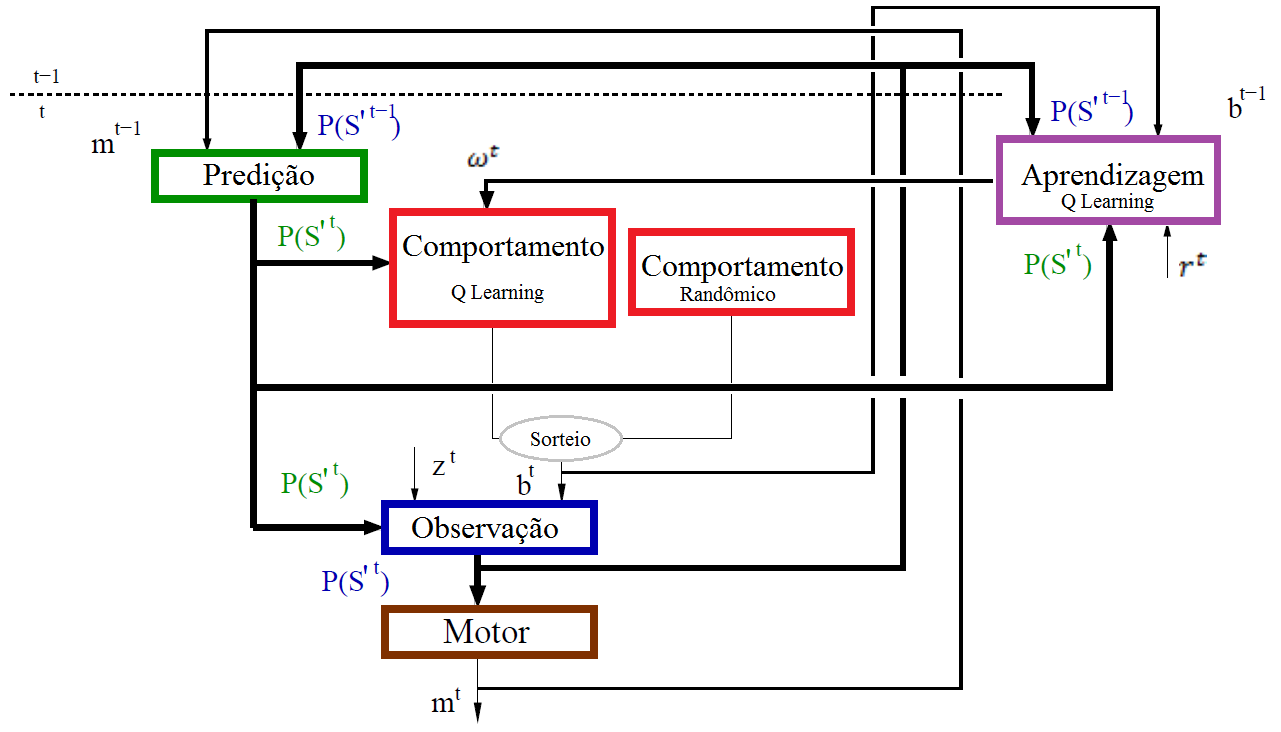
\includegraphics[width=150mm]{images/modelo_bayesiano_treino-tiago}
    \caption{\label{img:ModeloFinalTreinamento}Filtro Bayesiano utilizando Q Learning para Seleção de Comportamento. Durante treinamento.}
\end{figure}

Após acabar o treinamento, não temos mais a etapa de aprendizagem, ficando então com um modelo com apenas 4 etapas. Esse modelo pode ser representado pela figura \ref{img:ModeloFinalPosTreinamento}.

\begin{figure}[h!]
    \centering
    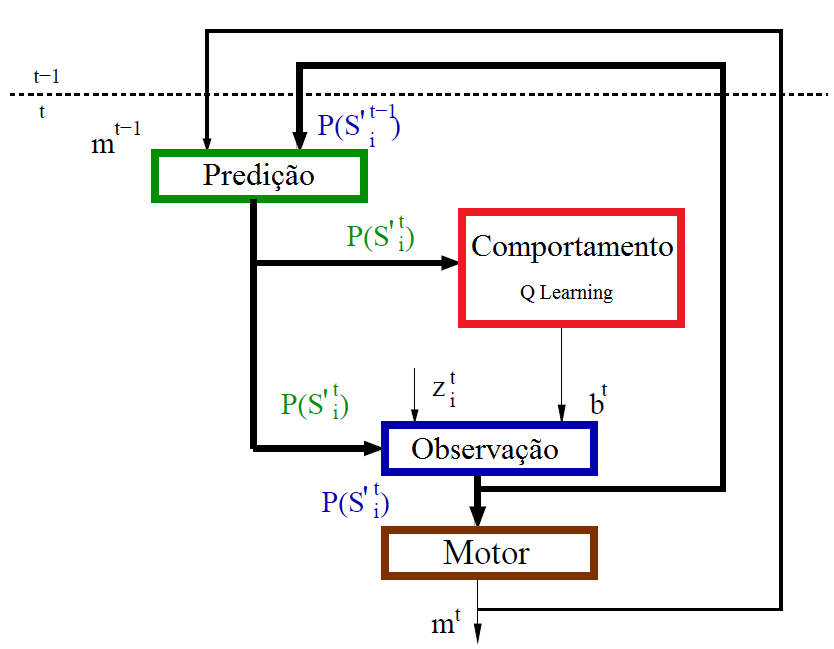
\includegraphics[width=120mm]{images/modelo_bayesiano_final-tiago}
    \caption{\label{img:ModeloFinalPosTreinamento}Filtro Bayesiano utilizando Q Learning para Seleção de Comportamento. Após treinamento completo.}
\end{figure}

\subsubsection{Predição} \label{subsubsection:ModeloFinalPredicao}

Nessa etapa, a partir da ação escolhida no período anterior de tempo, se faz uma estimativa de qual será o estado após sua execução.

\begin{equation}
    P \left( S^t S_b^t \mid z^{0: t-1} b^{0: t-1} m^{0: t-1} \pi_f \right) \propto \sum\limits_{S^{t-1} S_b^{t-1}}
        \left(
            \begin{array}{l}
                P \left( S^t \mid S^{t-1} m^{t-1} \pi_f \right) \times P \left( S_b^t \mid \pi_f \right) \\
                \times P \left( m^{t-1} \mid S^{t-1} S_b^{t-1} m^{t-2} \pi_f \right)\\
                \times P \left( S^{t-1} S_b^{t-1} \mid z^{0: t-1} b^{0: t-1} m^{0: t-2} \pi_f \right)
            \end{array}
        \right)
\end{equation}


\subsubsection{Escolha de comportamento}

Essa etapa é onde a escolha do comportamento acontece. Ela pode ter dois métodos distintos, um durante a fase de treinamento e outro após acabar a aprendizagem.

Durante a aprendizagem se utiliza uma exploração gulosa, descrita no tópico \ref{subsection:EscolhaDeAçõesExploraçãoGulosa}, para a escolha do comportamento. Nela, primeiro se sorteia um número randômico $ x \in [0,1] $. Se esse número for menor que um fator de exploração $ \gamma $, se escolhe uma ação randômica entre todas as possíveis. No caso contrário, se escolhe uma ação da seguinte forma, que é como é feita a escolha após a aprendizagem ter acabado.

Primeiro se calcula a função à seguir para cada comportamento $ b \in B^t $ e para o conjunto de probabilidades%
\footnote{É importante ressaltar que $ a^t $ equivale ao conjunto de probabilidades $ P \left( S^t S_b^t \mid z^{0: t-1} b^{0: t-1} m^{0: t-1} \pi_f \right) $, obtido em \ref{subsubsection:ModeloFinalPredicao}.%
} $ a^t \in A^t $ de se encontrar em cada estado $ S^t $.

\begin{equation}
    	Q \left( a^t, B^t \right) = \omega^1 \cdot f^1 \left( a^t, B^t \right) + \omega^2 \cdot f^2 \left( a^t, B^t \right) + \cdots + \omega^n \cdot f^n \left( a^t, B^t \right)
\end{equation}

Depois, se escolhe um comportamento a partir desses valores calculados, sendo escolhido o que maximize essa função%
\footnote{Durante as etapas de aprendizagem se escolhe um comportamentos aleatório com uma probabilidade $ \gamma $, chamada parâmetro de exploração, para se explorar outros comportamentos.}.


\subsubsection{Observação}

A partir dos sensores presentes no robô e do valor $ b \in B $, obtido com o algoritmo de aprendizado, se atualiza o belief state do agente.

\begin{equation}
    P \left( S^t S_b^t \mid z^{0: t} b^{0: t} m^{0: t-1} \pi_f \right) \propto
        \left(
            \begin{array}{l}
                P \left( z^t \mid S^t \pi_f \right) \times P \left( b^t \mid S_b^t \pi_f \right) \\
                \times P \left( S^t S_b^t \mid z^{0: t-1} b^{0: t-1} m^{0: t-1} \pi_f \right)
            \end{array}
        \right)
\end{equation}


\subsubsection{Escolha de ação motora}

Por último se faz a seleção de uma ação a ser executada pelo robô. Para isso, calcula-se as probabilidade de se executar cada ação e se escolhe a com maior valor.

\begin{equation}
    P \left( M^t \mid z^{0: t} b^{0: t} m^{0: t-1} \pi_f \right) \propto \sum\limits_{S_i^t S_b^t}
        \left(
            \begin{array}{l}
                P \left( M^t \mid S^t S_b^t m^{t-1} \pi_f \right)\\
                \times P \left( S^t S_b^t \mid z^{0: t} b^{0: t} m^{0: t-1} \pi_f \right)
            \end{array}
        \right)
\end{equation}


\subsubsection{Aprendizagem}

Nessa etapa são atualizados os valores do modelo de seleção de comportamento $ Q \left( A, B \right) $ a partir de uma recompensa $ r $ recebida. Tendo posse dessa recompensa, das probabilidades $ a^{t-1} \in A^{t-1} $ do estado anterior e atual $ a^t \in A^t $ do sistema e de qual o comportamento $ b^{t-1} \in B^{t-1} $ escolhido no tempo anterior pelo algoritmo de aprendizagem, podemos atualizar os pesos $ \omega_i $ do sistema de aprendizagem, como descrito nas equações \ref{equation:ErroQPartiallyObservable} e \ref{equation:UpdateOmegaQPartiallyObservable}, reescritas aqui.

$$
	erro = r \left( a, b, a' \right) + \gamma \cdot \underset{b}{max} \left( Q^{t-1} \left( a', b' \right) \right) - Q^{t-1} \left( a, b \right)
$$

$$
	\omega_i^t = \omega_i^{t-1} + \alpha \cdot erro \cdot f_i \left( a, b \right)
$$



\section{Ambiente de testes e simulação} \label{section:AmbienteDeTestes}

Para poder testar as teorias aqui descritas foi utilizado uma plataforma de Pacman [referência http://ai.berkeley.edu/project\_overview.html], criada em Berkeley para suas aulas de inteligência artificial.

\begin{figure}[H]
    \centering
    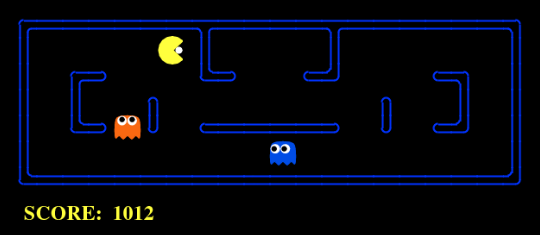
\includegraphics[width=120mm]{images/pacman_platform}
    \caption{\label{img:PlataformaSimulacaoPacman}Plataforma do jogo Pacman desenvolvida em Berkeley para aulas de IA.}
\end{figure}

A plataforma provê um sistema com informação completa%
\footnote{Todas as propriedades do jogo são conhecidas a todo momento, como por exemplo: posição do Pacman, posição dos fantasmas e localizações com ou se comida.%
} e sem erros na movimentação%
\footnote{Uma ação executada em um dado estado do sistema terá sempre o mesmo resultado.%
}. Essa plataforma foi programada em python e a integramos com ROS [refs ROS] para criar um sistema de forma mais generalizada. Utilizando ROS nós conectamos essa plataforma com um programa em C++, no qual foi programado o modelo de aprendizagem e seleção de comportamento proposto nesse trabalho.

A comunicação entre a plataforma em Python e o programa em C++ se deu a partir de quatro mensagens diferentes, as quais simulavam os sensores, atuadores e recompensas do sistema.

\begin{itemize}
	\item Posição do agente (Pacman) --- $ \left( x, y \right) \in \mathbb{R}^2 $
	\item Distância para os fantasmas --- $ \left( d_x, d_y \right) = \left( \Delta x, \Delta y \right) \in \mathbb{R}^2 $
	\item Ação a ser executada --- $ u \in \left\{Norte, Sul, Leste, Oeste, Esperar \right\} $
	\item Recompensa recebida do ambiente --- $ r \in \mathbb{R} $
\end{itemize}

Para simular erros de sensoriamento, comuns em aplicação de robótica móvel, antes de enviar essas informações são inseridos erros Gaussianos tanto na posição do agente (Pacman), quanto nas distâncias pros fantasmas. Para simular erros de atuação, foi inserido um erro na forma de atuação a ser executada também.

$$
	\left( x, y \right) = \left( x^*, y^* \right) + \left( \delta\left( 0, \sigma_{pacman} \right), \delta\left( 0, \sigma_{pacman} \right) \right)
$$

\begin{equation}
	\left( x, y \right) = \left( \delta\left( x^*, \sigma_{pacman} \right), \delta\left( y^*, \sigma_{pacman} \right) \right)
\end{equation}

Sendo:

\begin{itemize}
	\item $ \delta \left( \mu, \sigma \right) $ uma função que gera um número aleatório baseado numa gaussiana com média $ \mu $ e desvio padrão $ 
sigma $;
	\item $ \sigma_{pacman} $ o desvio padrão do erro inserido na posição do agente;
	\item $ \left( x^*, y^* \right) $ a posição exata do agente.
\end{itemize}

Analogamente a distância ``vista'' dos fantasmas ficou:

\begin{equation}
	\left( d_x, d_y \right) = \left( \delta\left( d_x^*, \sigma_{dist\_fant} \right), \delta\left( d_y^*, \sigma_{dist\_fant} \right) \right)
\end{equation}

A atuação tem um conjunto de valores possível tal que $ u \in U = \left\{ Norte, Sul, Leste, Oeste, Parar \right\} $. Como ela possui um valor discreto e não numérico, não inserimos um erro gaussiano gaussiano nela. Ela é recebida pela plataforma de simulação e um erro é inserido nela de acordo com a função a seguir:

\begin{algorithm}[H]
	\caption{Erro na Atuação} \label{algorithm:ErroAtuacao}
	\begin{algorithmic}[1]
		\Procedure{ExecutarAção}{\textit{ação\_escolhida}}
			\State $\textit{numero\_randomico} \gets \text{random }\textit{numero}$
			\If {$\textit{numero\_randomico} > \text{FATOR\_DE\_ACERTO} $ }
				\State $\textit{acao\_randomica} \gets \text{random }\textit{ação} \in \textit{Ações}-\textit{\{ação\_escolhida\}}$
				\State \Return $\textit{acao\_randomica}$
			\Else
				\State \Return $\textit{ação\_escolhida}$
			\EndIf
		\EndProcedure
	\end{algorithmic}
\end{algorithm}

Ou seja, a atuação tem uma chance $ \nu_{atuacao} = \textit{FATOR\_DE\_ACERTO} $ de ser executada como experado. Ela tem também uma proabilidade $ 1 - \nu_{atuacao} $ de ser selecionada uma ação randômica diferente da escolhida.

A recompensa $ r $ é, por sua vez, enviada da plataforma de simulação para o sistema de aprendizagem. Nela não inserimos qualquer forma de erro e ela representa a diferença de pontuação entre a etapa atual e a anterior no jogo, ou seja, a pontuação recebida pela última ação executada.


\section{Testes realizados} \label{section:TestesRealizados}

Nessa seção explicaremos como foi realizado cada teste presente na análise de dados e quais parâmetros foram utilizados.

\subsection{3 Comportamentos no mapa pequeno (Teste 1)}

Nesse primeiro teste foi feito no mapa pequeno, mostrado na figura \ref{}, e foram utilizados apenas três comportamentos:

\begin{itemize}
	\item Parar
	\item Comer
	\item Fugir
\end{itemize}

\subsubsection{Parâmetros Utilizados}

\begin{multicols}{2}

Num. partidas%
\footnote{Número de partidas executadas%
} = 2300

Num. treinos%
\footnote{Número de partidas usadas para treinamento%
} = 2000

Num. Greedy%
\footnote{Número de partidas em que foi utilizada exploração gulosa. Como explicado no tópico \ref{subsection:EscolhaDeAçõesExploraçãoGulosa}%
} = 500

$ \beta%
\footnote{Fator de exploração gulosa utilizado.%
} = 1 - \left( \frac{n}{Num. Greedy} \right) $

$ \alpha%
\footnote{Fator de Aprendizagem%
} = 0.002 $

$ \gamma%
\footnote{Fator de Desconto%
} = 0.99 $

$ \sigma_{pacman}%
\footnote{Desvio padrão do erro gaussiano da posição recebida do Pacman%
} = 0.5 $

$ \sigma_{dist\_fant}%
\footnote{Desvio padrão do erro gaussiano da distância recebida para os Fantasmas%
} = 0.5 $

$ \nu_{atuação}%
\footnote{Fator de Acerto na movimentação do Pacman. Descrito no algorítmo \ref{algorithm:ErroAtuacao} na seção \ref{section:AmbienteDeTestes}%
} = 0.9 $

\end{multicols}

Sendo $ n $ o número da partida sendo jogada.

\subsubsection{Comportamentos Utilizados}

Os comportamentos utilizados foram: parar, comer e fugir. Ou seja, $$ b \in B = \left\{ Ficar\_Parado, Comer, Fugir \right\} $$ $$ s_b \in S_b = \left\{ Estado\_Parar, Estado\_Comer, Estado\_Fugir \right\} $$. Como explicado no tópico \ref{subsection:BayesComSelecaoDeComportamento} agora podemos ter três modelos de seleção de ação: 

\begin{equation}
    P \left( M^t \mid S^t S_b^t M^{t-1} \pi_f \right) = 
        \left\{
            \begin{array}{l}
                P \left( M^t \mid S^t \left[ S_b^t=Estado\_Parar \right] M^{t-1} \pi \right) \\
                P \left( M^t \mid S^t \left[ S_b^t=Estado\_Comer \right] M^{t-1} \pi \right) \\
                P \left( M^t \mid S^t \left[ S_b^t=Estado\_Fugir \right] M^{t-1} \pi \right)
            \end{array}
        \right.
\end{equation}

Abaixo é dada uma descrição mais detalhada de como cada modelo é feito.

\subsubsection*{Parar}

Esse é comportamento o comportamento mais simples, tendo como modelo de seleção de ação:

\begin{equation}
    P \left( m^t \mid S^t \left[ S_b^t = Estado\_Parar \right] M^{t-1} \pi_f \right) = 
        \left\{
            \begin{array}{l l}
                0.99 & \text{se }m^t = Parar \\
                0.0025 & \text{senão}
            \end{array}
        \right.
\end{equation}

\subsubsection*{Comer}

Para esse comportamento foi utilizado um modelo mais complexo em que, para um dado estado de $ S^t $ se calculava uma ação com o seguinte algoritmo:

\begin{algorithm}[H]
	\caption{Escolher Ação Comer} \label{algorithm:SelecaoDeAcaoComer}
	\begin{algorithmic}[1]
		\Procedure{EscolherAçãoComer}{\textit{estado}}
			\State $\textit{pos\_comida} \gets \text{posição }\textit{comida\_mais\_proxima} $
			\State $\textit{pos\_pacman} \gets \text{posição }\textit{pacman} $
			\State $\textit{dist\_atual} \gets \text{dist} \left( \textit{pos\_comida}, \textit{pos\_pacman} \right) $
			\For{Ação $ in $ Ações}
				\State $\textit{nova\_pos\_pacman} \gets \text{executa} \left( \textit{pos\_pacman}, \textit{Ação} \right) $
				\If{$ \text{dist} \left( \textit{pos\_comida}, \textit{nova\_pos\_pacman} \right) < \textit{dist\_atual} $ }
					\State \Return $ \textit{Ação} $
				\EndIf 
			\EndFor
			\State \Return $ \textit{Erro} $
		\EndProcedure
	\end{algorithmic}
\end{algorithm}

Depois de calculado essa ação para um estado $ s^t \in S^t $, utilizamos um modelo parecido com o para o comportamento parado.

\begin{equation}
    P \left( m^t \mid s^t \left[ S_b^t = Estado\_Comer \right] M^{t-1} \pi_f \right) = 
        \left\{
            \begin{array}{l l}
                0.99 & \text{se }m^t = \textit{Ação} \\
                0.0025 & \text{senão}
            \end{array}
        \right.
\end{equation}

\subsubsection*{Fugir}

Para esse comportamento foi utilizado um formato parecido com o de comer, mas com um modelo diferente. Para um dado estado de $ S^t $ se calculava uma ação com o seguinte algoritmo:

\begin{algorithm}[H]
	\caption{Escolher Ação Fugir} \label{algorithm:SelecaoDeAcaoFugir}
	\begin{algorithmic}[1]
		\Procedure{EscolherAçãoFugir}{\textit{estado}}
			\State $\textit{pos\_fantasma} \gets \text{posição }\textit{fantasma\_mais\_proximo} $
			\State $\textit{pos\_pacman} \gets \text{posição }\textit{pacman} $
			\State $\textit{dist\_atual} \gets \text{dist} \left( \textit{pos\_fantasma}, \textit{pos\_pacman} \right) $
			\For{Ação $ in $ Ações}
				\State $\textit{nova\_pos\_pacman} \gets \text{executa} \left( \textit{pos\_pacman}, \textit{Ação} \right) $
				\If{$ \text{dist} \left( \textit{pos\_fantasma}, \textit{nova\_pos\_pacman} \right) < \textit{dist\_atual} $ }
					\State \Return $ \textit{Ação} $
				\EndIf 
			\EndFor
			\State \Return $ \textit{Erro} $
		\EndProcedure
	\end{algorithmic}
\end{algorithm}

Depois de calculado essa ação para um estado $ s^t \in S^t $, assim como para o comportamento anterior, utilizamos um modelo parecido com o para o comportamento parado.

\begin{equation}
    P \left( m^t \mid s^t \left[ S_b^t = Estado\_Fugir \right] M^{t-1} \pi_f \right) = 
        \left\{
            \begin{array}{l l}
                0.99 & \text{se }m^t = \textit{Ação} \\
                0.0025 & \text{senão}
            \end{array}
        \right.
\end{equation}

\subsubsection{Vetor de Características Utilizado}

\subsubsection*{Bias}

Essa é uma característica que sempre está presente nesse vetor. Ela tem um valor igual a $ 1.0 $ e seu peso $ \omega $ indica quão bom esse comportamento é, independente da situação atual.

$$ f_1 = 1.0 $$

\subsubsection*{Distância para Provável Comida mais Próxima} \label{subsubsection:DistProvavelComida}

Essa característica indica qual a distância até a posição mais próxima em que é provável existir uma comida. Ela pode ser obtida a partir do algoritmo a seguir:

\begin{algorithm}[H]
	\caption{Obter Característica Distancia Comida} \label{algorithm:ObterCaracteristicaDistanciaComida}
	\begin{algorithmic}[1]
		\Procedure{ObterCaracterísticaDistanciaComida}{\textit{probabilidades\_estados}}
			\State $\textit{max\_prob} \gets 0.0 $
			\For{Posição $ in $ Posições}
				\State $\textit{prob\_comida} \gets \text{probabilidade de comida } \left( \textit{Posição} \right) $
				\If{ $ \textit{prob\_comida} > \textit{max\_prob} $ }
					\State $\textit{max\_prob} \gets \textit{prob\_comida} $
				\EndIf 
			\EndFor
			\For{Posição $ in $ Posições}
				\State $\textit{prob\_comida} \gets \text{probabilidade de comida } \left( \textit{Posição} \right) $
				\If{ $ \textit{prob\_comida} > \frac{\textit{max\_prob} }{2} $ }
					\State $ \text{Prob\_Posições } append \text{ Posição} $
				\EndIf 
			\EndFor
			\State $\textit{pos\_comida} \gets \text{mais proxima }\textit{posição} \in \text{Prob\_Posições} $
			\State $\textit{pos\_pacman} \gets \text{posição }\textit{pacman} $
			\State \Return $ \text{dist} \left( \textit{pos\_comida}, \textit{pos\_pacman} \right) $
		\EndProcedure
	\end{algorithmic}
\end{algorithm}

Tendo um conjunto de probabilidades $ a \in A $ para os estados:

$$ f_2 = ObterCaracteristicaDistanciaComida \left( a \right) $$

\subsubsection*{Soma das Probabilidades de Fantasmas a menos de 4 Movimentos}

Essa característica é obtida a partir da soma das probabilidades de haver fantasmas a 3 movimentos de distância, ou menos, podendo então ir de $ \left[ 0, num\_fantasmas \cdot 100\% \right] $.

\begin{algorithm}[H]
	\caption{Obter Característica Probabilidades Fantasmas} \label{algorithm:ObterCaracteristicaProbabilidadesFantasmas}
	\begin{algorithmic}[1]
		\Procedure{ObterCaracterísticaProbFantasmas}{\textit{probabilidades\_estados}}
			\State $\textit{total} \gets 0.0 $
			\For{Posição $ in $ Posições}
				\For{Posição2 $ in $ Posições}
					\If{ $ \text{dist} \left( \textit{Posição} , \textit{Posição2} \right) < 4 $ }
						\State $\textit{prob\_pacman} \gets \text{probabilidade pacman } \left( \textit{Posição} \right) $
						\For{Fantasma $ in $ Fantasmas}
							\State $\textit{prob\_fantasma} \gets \text{probabilidade Fantasma } \left( \textit{Posição2} \right) $
							\State $\textit{prob\_fantasma\_normal} \gets \text{probabilidade normal } \left( \textit{Fantasma} \right) $
							\State $\textit{total} \gets \textit{total} + \textit{prob\_pacman}  \cdot \textit{prob\_fantasma} \cdot \textit{prob\_fantasma\_normal} $
						\EndFor
					\EndIf
				\EndFor
			\EndFor
			\State \Return $ \textit{total} $
		\EndProcedure
	\end{algorithmic}
\end{algorithm}

$$ f_3 = ObterCaracteristicaProbFantasmas \left( a \right) $$


\subsection{3 Comportamentos no mapa original (Teste 2)}

\subsection{5 Comportamentos no mapa pequeno (Teste 3)}

Esse teste foi feito no mapa pequeno, mostrado na figura \ref{}, e nele foram utilizados apenas cinco comportamentos:

\begin{itemize}
	\item Parar
	\item Comer
	\item Fugir
	\item Comer Cápsula
	\item Caçar
\end{itemize}

\subsubsection{Parâmetros Utilizados}

\subsubsection{Comportamentos Utilizados}


Os comportamentos utilizados foram: parar, comer, fugir, comer cápsula e caçar. Ou seja:

$$ b \in B = \left\{ Ficar\_Parado, Comer, Fugir, Comer\_Capsula, \textit{Caçar} \right\} $$

$$ s_b \in S_b = 
        \left\{
            \begin{array}{l}
                Estado\_Parar, \\
                Estado\_Comer, \\
                Estado\_Fugir, \\
                Estado\_Comer\_Capsula, \\
                \textit{Estado\_Caçar}
            \end{array}
        \right\}
         $$

Como explicado no tópico \ref{subsection:BayesComSelecaoDeComportamento}, e analogamente ao visto para três comportamentos, agora podemos ter cinco modelos de seleção de ação: 

\begin{equation}
    P \left( M^t \mid S^t S_b^t M^{t-1} \pi_f \right) = 
        \left\{
            \begin{array}{l}
                P \left( M^t \mid S^t \left[ S_b^t=Estado\_Parar \right] M^{t-1} \pi \right) \\
                P \left( M^t \mid S^t \left[ S_b^t=Estado\_Comer \right] M^{t-1} \pi \right) \\
                P \left( M^t \mid S^t \left[ S_b^t=Estado\_Fugir \right] M^{t-1} \pi \right) \\
                P \left( M^t \mid S^t \left[ S_b^t=Estado\_Comer\_Capsula \right] M^{t-1} \pi \right) \\
                P \left( M^t \mid S^t \left[ S_b^t=\textit{Estado\_Caçar} \right] M^{t-1} \pi \right)
            \end{array}
        \right.
\end{equation}

Abaixo é dada uma descrição mais detalhada de como cada modelo é feito.

\subsubsection*{Parar}

\subsubsection*{Comer}

\subsubsection*{Fugir}

\subsubsection*{Comer Cápsula}

\subsubsection*{Caçar}

\subsubsection{Vetor de Características Utilizado}

\subsubsection*{Bias}

Já descrito.

Essa é uma característica que sempre está presente nesse vetor. Ela tem um valor igual a $ 1.0 $ e seu peso $ \omega $ indica quão bom esse comportamento é, independente da situação atual.

$$ f_1 = 1.0 $$

\subsubsection*{Distância para Provável Comida mais Próxima}

Já descrito.

$$ f_2 = ObterCaracteristicaDistanciaComida \left( a \right) $$

\subsubsection*{Soma das Probabilidades de Fantasmas a menos de 4 Movimentos}

Já descrito.

$$ f_3 = ObterCaracteristicaProbFantasmas \left( a \right) $$

\subsubsection*{Soma das Probabilidades de Fantasmas Brancos a menos de 4 Movimentos}

Essa característica é obtida a partir da soma das probabilidades de haver fantasmas a 3 movimentos de distância, ou menos, podendo então ir de $ \left[ 0, num\_fantasmas \cdot 100\% \right] $.

\begin{algorithm}[H]
	\caption{Obter Característica Probabilidades Fantasmas Brancos} \label{algorithm:ObterCaracteristicaProbabilidadesFantasmasBrancos}
	\begin{algorithmic}[1]
		\Procedure{ObterCaracterísticaProbFantasmasBrancos}{\textit{probabilidades\_estados}}
			\State $\textit{total} \gets 0.0 $
			\For{Posição $ in $ Posições}
				\For{Posição2 $ in $ Posições}
					\If{ $ \text{dist} \left( \textit{Posição} , \textit{Posição2} \right) < 4 $ }
						\State $\textit{prob\_pacman} \gets \text{probabilidade pacman } \left( \textit{Posição} \right) $
						\For{Fantasma $ in $ Fantasmas}
							\State $\textit{prob\_fantasma} \gets \text{probabilidade Fantasma } \left( \textit{Posição2} \right) $
							\State $\textit{prob\_fantasma\_branco} \gets \text{probabilidade branco } \left( \textit{Fantasma} \right) $
							\State $\textit{total} \gets \textit{total} + \textit{prob\_pacman}  \cdot \textit{prob\_fantasma} \cdot \textit{prob\_fantasma\_branco} $
						\EndFor
					\EndIf
				\EndFor
			\EndFor
			\State \Return $ \textit{total} $
		\EndProcedure
	\end{algorithmic}
\end{algorithm}

$$ f_4 = ObterCaracteristicaProbFantasmasBrancos \left( a \right) $$

\subsubsection*{Probabilidade de Existir Fantasma Branco}

Essa característica é obtida a partir da probabilidade de existir um fantasma branco no ambiente.

$$ f_5 = P \left( fantasma\_branco \mid a \right) $$

\subsubsection*{Distância para Provável Capsula mais Próxima} \label{oi}

Essa característica indica qual a distância até a posição mais próxima em que é provável existir uma capsula. Ela pode ser obtida a partir do algoritmo a seguir, que é análogo ao algoritmo \ref{algorithm:ObterCaracteristicaDistanciaComida} do tópico \ref{subsubsection:DistProvavelComida}:

\begin{algorithm}[H]
	\caption{Obter Característica Distancia Capsula} \label{algorithm:ObterCaracteristicaDistanciaCapsula}
	\begin{algorithmic}[1]
		\Procedure{ObterCaracterísticaDistanciaCapsula}{\textit{probabilidades\_estados}}
			\State $\textit{max\_prob} \gets 0.0 $
			\For{Posição $ in $ Posições}
				\State $\textit{prob\_capsula} \gets \text{probabilidade de capsula } \left( \textit{Posição} \right) $
				\If{ $ \textit{prob\_capsula} > \textit{max\_prob} $ }
					\State $\textit{max\_prob} \gets \textit{prob\_capsula} $
				\EndIf 
			\EndFor
			\For{Posição $ in $ Posições}
				\State $\textit{prob\_capsula} \gets \text{probabilidade de capsula } \left( \textit{Posição} \right) $
				\If{ $ \textit{prob\_capsula} > \frac{\textit{max\_prob} }{2} $ }
					\State $ \text{Prob\_Posições } append \text{ Posição} $
				\EndIf 
			\EndFor
			\State $\textit{pos\_capsula} \gets \text{mais proxima }\textit{posição} \in \text{Prob\_Posições} $
			\State $\textit{pos\_pacman} \gets \text{posição }\textit{pacman} $
			\State \Return $ \text{dist} \left( \textit{pos\_capsula}, \textit{pos\_pacman} \right) $
		\EndProcedure
	\end{algorithmic}
\end{algorithm}

Tendo um conjunto de probabilidades $ a \in A $ para os estados:

$$ f_2 = ObterCaracteristicaDistanciaCapsula \left( a \right) $$

\subsection{5 Comportamentos no mapa original (Teste 4)}
